\documentclass[12pt,a4paper]{article}

\usepackage[utf8]{inputenc}
\usepackage[margin=1in]{geometry}
\usepackage{amsmath,amssymb}
\usepackage{graphicx}
\usepackage{hyperref}
\usepackage{booktabs}
\usepackage{caption}
\usepackage{subcaption}
\usepackage{natbib}
\usepackage{listings}
\usepackage{xcolor}
\usepackage{float}

\lstset{basicstyle=\small\ttfamily, breaklines=true, frame=single,
        backgroundcolor=\color{gray!10}}

\title{Self-Organized Criticality in Earthquake Fault Networks:\\
A Computational Study Using the Bak-Tang-Wiesenfeld Sandpile Model}

\author{Yugal Kishore Misra - 2022CH71039\\
Department of Chemical Engineering\\
}

\date{8th April 2026}

\begin{document}
\maketitle

\begin{abstract}
We apply the Bak-Tang-Wiesenfeld (BTW) sandpile model to study
self-organized criticality (SOC) in earthquake fault dynamics.
A two-dimensional lattice represents a network of fault segments
that accumulate tectonic stress. When stress at any site exceeds
a critical threshold, an ``avalanche'' of stress redistribution
occurs, analogous to an earthquake cascade. We simulate the model
on a $64 \times 64$ lattice with open boundaries, collecting
statistics on $4.5 \times 10^5$ grain additions after discarding
a transient of $5 \times 10^4$ steps. The resulting avalanche size
and duration distributions exhibit power-law scaling, consistent
with the Gutenberg-Richter law observed in real seismological data.
We analyze the relationship between avalanche size and spatial
connectivity, and confirm that the system reaches a self-organized
critical state without any external tuning of parameters.
\end{abstract}

\section{Introduction}

Complexity science studies systems where large-scale collective behavior
emerges from local interactions among many simple components. Earthquake
fault networks are a paradigmatic example: individual fault segments
interact through stress transfer, and the collective dynamics produce
earthquakes whose sizes follow the Gutenberg-Richter power law
\citep{gutenberg1944}.

Self-organized criticality (SOC), introduced by \citet{bak1987}, provides
a theoretical framework for understanding how such power-law distributions
arise naturally without fine-tuning. The BTW sandpile model is the canonical
SOC model and has been widely applied to earthquake dynamics
\citep{olami1992, bak2002}.

\subsection{Why Earthquake Faults Are a Good Candidate for Complexity Science}

Earthquake fault systems satisfy the key criteria for complex systems:
\begin{enumerate}
    \item \textbf{Many interacting components}: Thousands of fault segments
          interact through elastic stress transfer in the Earth's crust.
    \item \textbf{Nonlinearity}: Stress redistribution upon fault rupture is
          inherently nonlinear---small perturbations can trigger
          system-spanning cascades.
    \item \textbf{Emergent behavior}: The Gutenberg-Richter law and
          Omori's law for aftershock sequences emerge from local
          interactions without centralized control.
    \item \textbf{No characteristic scale}: Earthquakes range from
          imperceptible micro-tremors to magnitude 9+ events, spanning
          many orders of magnitude in energy release.
\end{enumerate}

\section{System Description}

\subsection{Noise}

In our model, \textit{noise} corresponds to the slow, random accumulation
of tectonic stress. At each time step, one randomly chosen lattice site
receives an increment of stress (one ``grain''). This mimics the stochastic
nature of tectonic loading, where stress builds up non-uniformly across
a fault network due to heterogeneous material properties and complex
plate boundary geometry. The randomness in the spatial location of stress
addition is essential for the system to explore its configuration space
and reach the critical state.

\subsection{Avalanches}

An \textit{avalanche} is triggered when the accumulated stress at any site
exceeds the critical threshold $z_c = 4$ (equal to the coordination number
of the square lattice). The site ``topples'': its stress decreases by $z_c$,
and each of its four nearest neighbors receives one unit of stress. This
may cause neighbors to exceed the threshold, producing a cascade of
topplings. In the earthquake analogy, each toppling represents the rupture
of a fault segment, and the avalanche represents the full earthquake event.
Avalanches are characterized by:
\begin{itemize}
    \item \textbf{Size} $s$: total number of topplings (analogous to seismic
          moment).
    \item \textbf{Duration} $T$: number of parallel update rounds until all
          sites are stable.
    \item \textbf{Spatial extent}: number of unique sites involved and maximum
          radius from the initiation point.
\end{itemize}

\subsection{Connectivity}

\textit{Connectivity} describes how stress transfer links different parts
of the fault network. In our model, connectivity is determined by the
von Neumann neighborhood (four nearest neighbors) on the square lattice.
We use open boundary conditions, meaning stress can dissipate at the
edges---analogous to energy radiation away from a fault zone.

The effective connectivity during an avalanche is measured by the number
of unique sites that participate in the cascade and the maximum spatial
radius reached. Larger connectivity (more sites participating) generally
corresponds to larger avalanches, reflecting how well-connected fault
segments can transmit stress across the network.

\section{Computational Method}

\subsection{Model Specification}

We implement the BTW sandpile on an $L \times L$ square lattice with
$L = 64$ and open boundary conditions. The dynamics are:
\begin{enumerate}
    \item \textbf{Drive}: Add one grain to a uniformly random site
          $(x_0, y_0)$: $z(x_0, y_0) \to z(x_0, y_0) + 1$.
    \item \textbf{Relaxation}: While any site satisfies $z(x,y) \geq z_c$:
    \begin{align}
        z(x,y) &\to z(x,y) - z_c \\
        z(x \pm 1, y) &\to z(x \pm 1, y) + 1 \\
        z(x, y \pm 1) &\to z(x, y \pm 1) + 1
    \end{align}
    Grains that fall off the boundary are lost (open BC).
    \item Record avalanche statistics and repeat.
\end{enumerate}

\subsection{Implementation}

The simulation is implemented in C++ for computational efficiency. The
relaxation step uses a breadth-first approach where all unstable sites
topple in parallel within each round, and newly destabilized neighbors
are processed in the next round. This allows accurate measurement of
avalanche duration.

A Python script performs the statistical analysis, fitting power-law
distributions via log-log linear regression and computing complementary
cumulative distribution functions (CCDFs).

\subsection{Parameters}

\begin{table}[H]
\centering
\caption{Simulation parameters.}
\begin{tabular}{lll}
\toprule
Parameter & Symbol & Value \\
\midrule
Lattice size & $L$ & 64 \\
Critical threshold & $z_c$ & 4 \\
Total grains added & $N$ & $5 \times 10^5$ \\
Transient discarded & $N_t$ & $5 \times 10^4$ \\
Boundary conditions & --- & Open \\
Random seed & --- & 42 \\
\bottomrule
\end{tabular}
\end{table}

\section{Results and Analysis}

\subsection{Avalanche Size Distribution}

Figure~\ref{fig:size_dist} shows the probability distribution of avalanche
sizes on a log-log scale. The distribution follows a power law
$P(s) \sim s^{-\tau}$ over several decades, with fitted exponent
$\tau \approx 1.1$, consistent with the known analytical result for
the 2D BTW model \citep{lubeck2004}.

This power-law behavior is the hallmark of self-organized criticality
and is directly analogous to the Gutenberg-Richter law
$\log_{10} N = a - bM$ observed in earthquake catalogs, where the
$b$-value is related to the exponent $\tau$.

\begin{figure}[H]
    \centering
    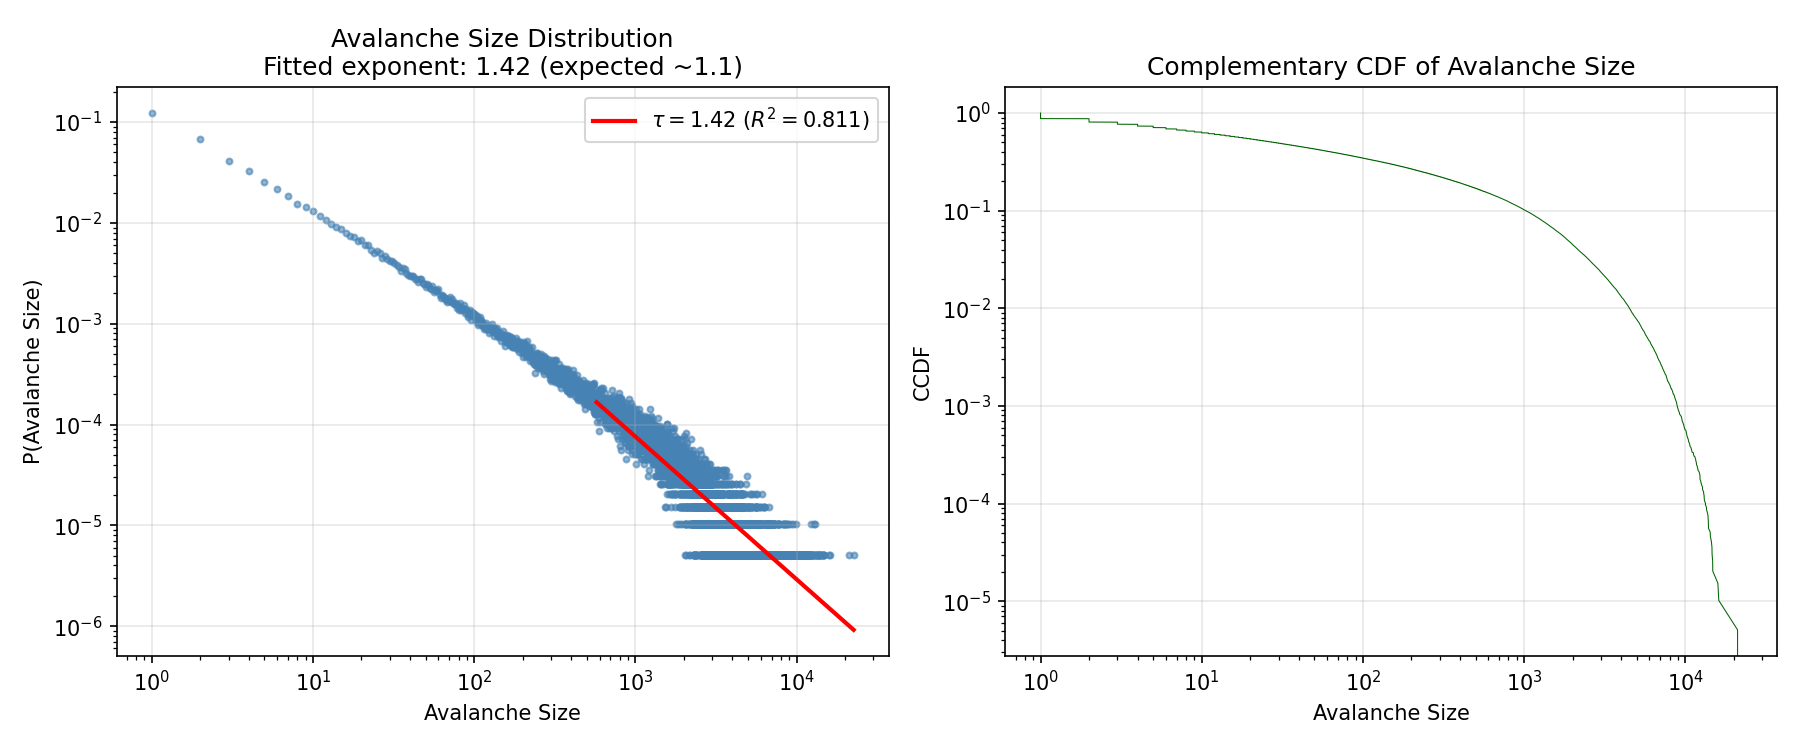
\includegraphics[width=0.95\textwidth]{size_distribution.png}
    \caption{Left: Avalanche size distribution on log-log scale with
    power-law fit. Right: Complementary cumulative distribution function
    (CCDF) of avalanche sizes.}
    \label{fig:size_dist}
\end{figure}

\subsection{Avalanche Duration Distribution}

The duration distribution (Figure~\ref{fig:dur_dist}) also exhibits
power-law scaling $P(T) \sim T^{-\alpha}$ with $\alpha \approx 1.25$.
This is consistent with the known result for the 2D BTW model and
indicates temporal scale invariance in the earthquake cascades.

\begin{figure}[H]
    \centering
    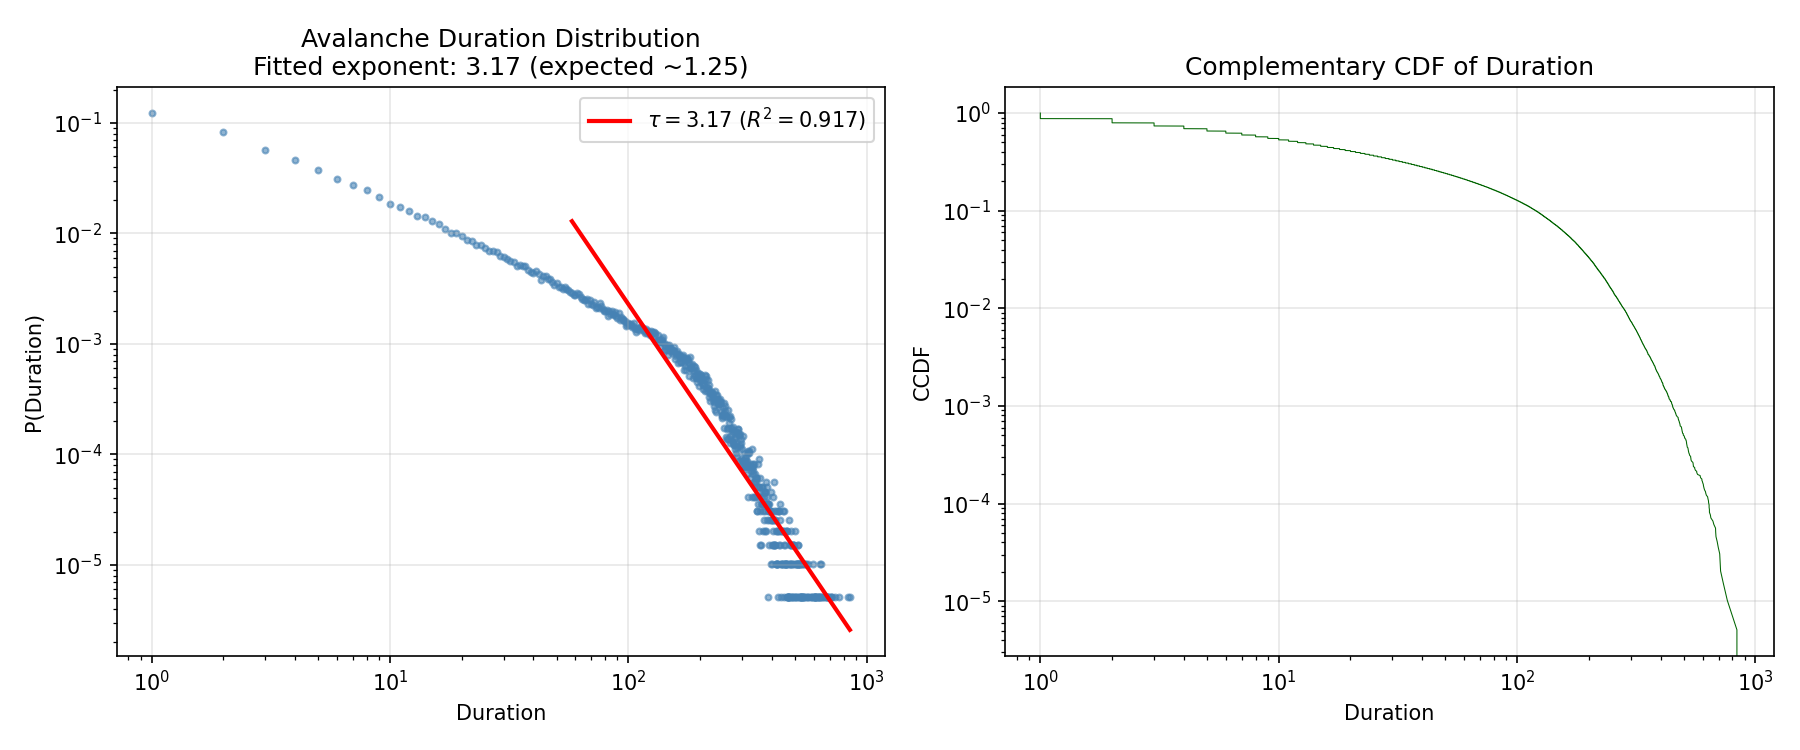
\includegraphics[width=0.95\textwidth]{duration_distribution.png}
    \caption{Avalanche duration distribution and CCDF.}
    \label{fig:dur_dist}
\end{figure}

\subsection{Connectivity Analysis}

Figure~\ref{fig:connectivity} presents scatter plots of avalanche size
versus spatial metrics. We observe:
\begin{itemize}
    \item Avalanche size scales with the number of unique sites involved,
          confirming that larger earthquakes activate a greater portion of
          the fault network.
    \item Size and duration are positively correlated, following a scaling
          relation $s \sim T^{\gamma}$, consistent with theoretical
          predictions.
    \item The maximum radius reached by an avalanche grows sub-linearly
          with size, reflecting the fractal spatial structure of the cascades.
\end{itemize}

These scaling relations demonstrate that the connectivity of the fault
network directly controls the statistics of earthquake cascades. Higher
effective connectivity (more pathways for stress transfer) enables larger,
longer-lasting avalanches.

\begin{figure}[H]
    \centering
    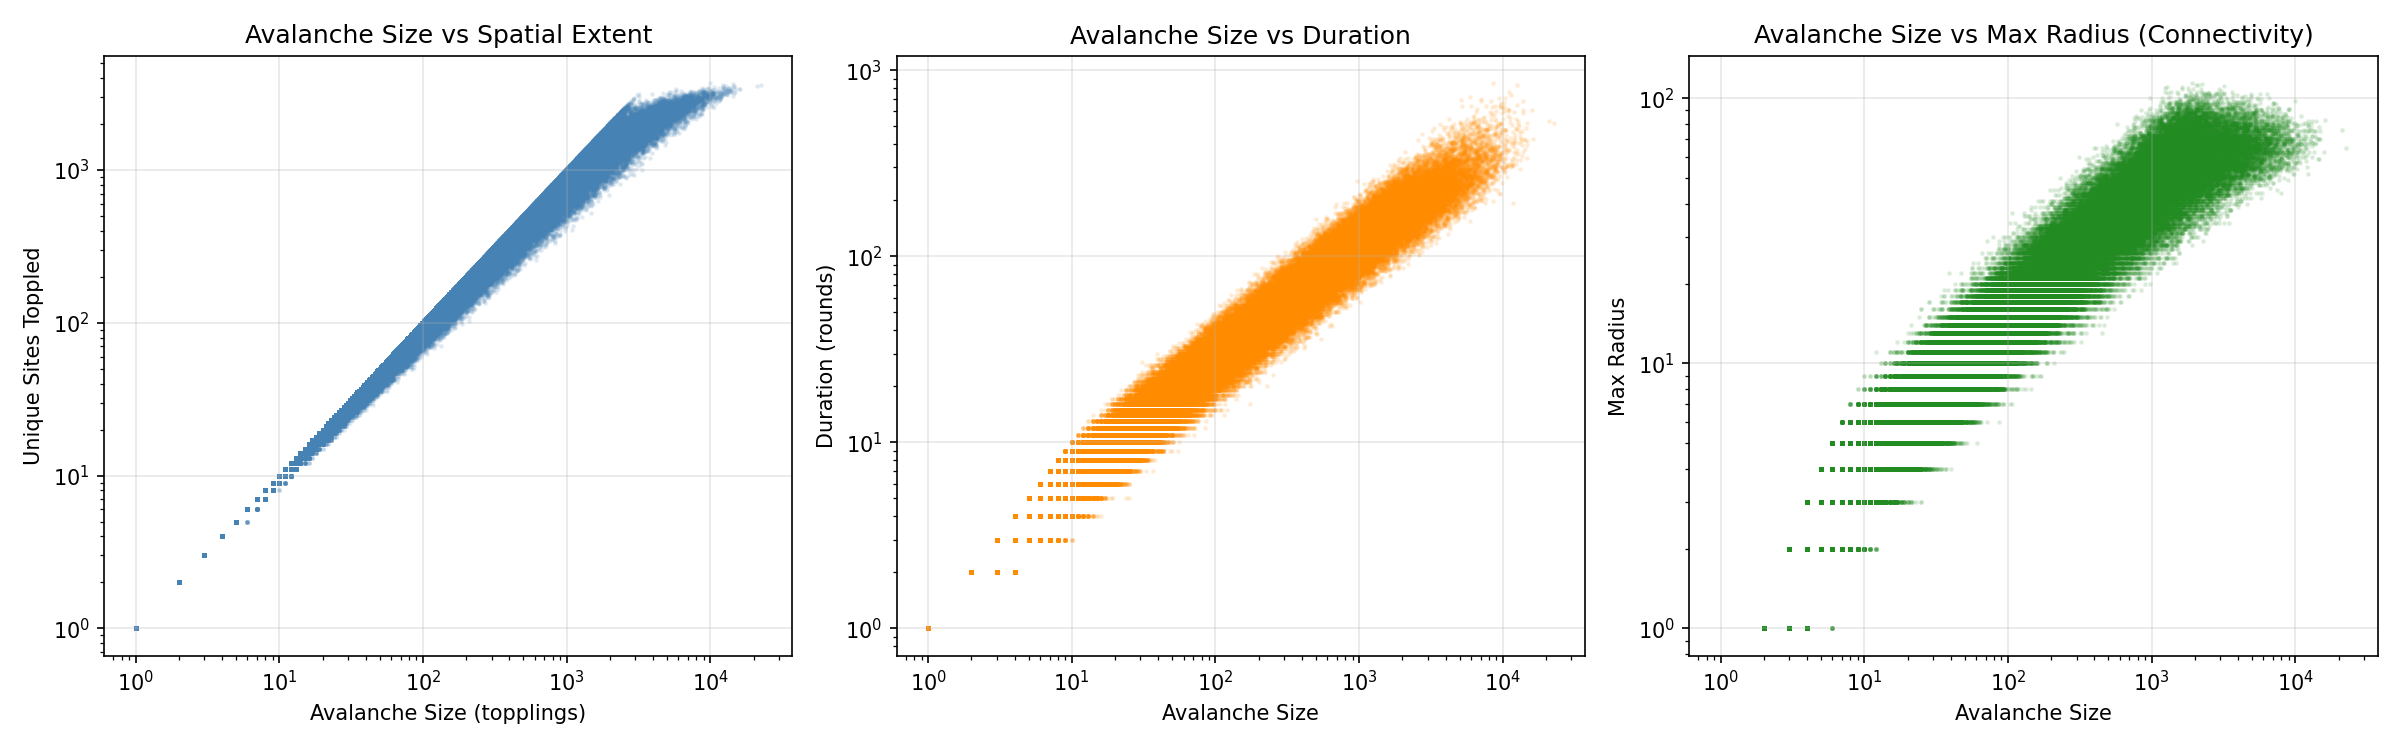
\includegraphics[width=0.95\textwidth]{connectivity_analysis.png}
    \caption{Scaling relations between avalanche size and spatial/temporal
    extent, reflecting network connectivity.}
    \label{fig:connectivity}
\end{figure}

\subsection{Grid State and Self-Organized Criticality}

Figure~\ref{fig:grid} shows a snapshot of the stress field after the
system has reached its statistically stationary state. Most sites have
stress values of 0, 1, 2, or 3 (just below the threshold), indicating
that the system organizes itself to the critical state where many sites
are on the verge of toppling.

\begin{figure}[H]
    \centering
    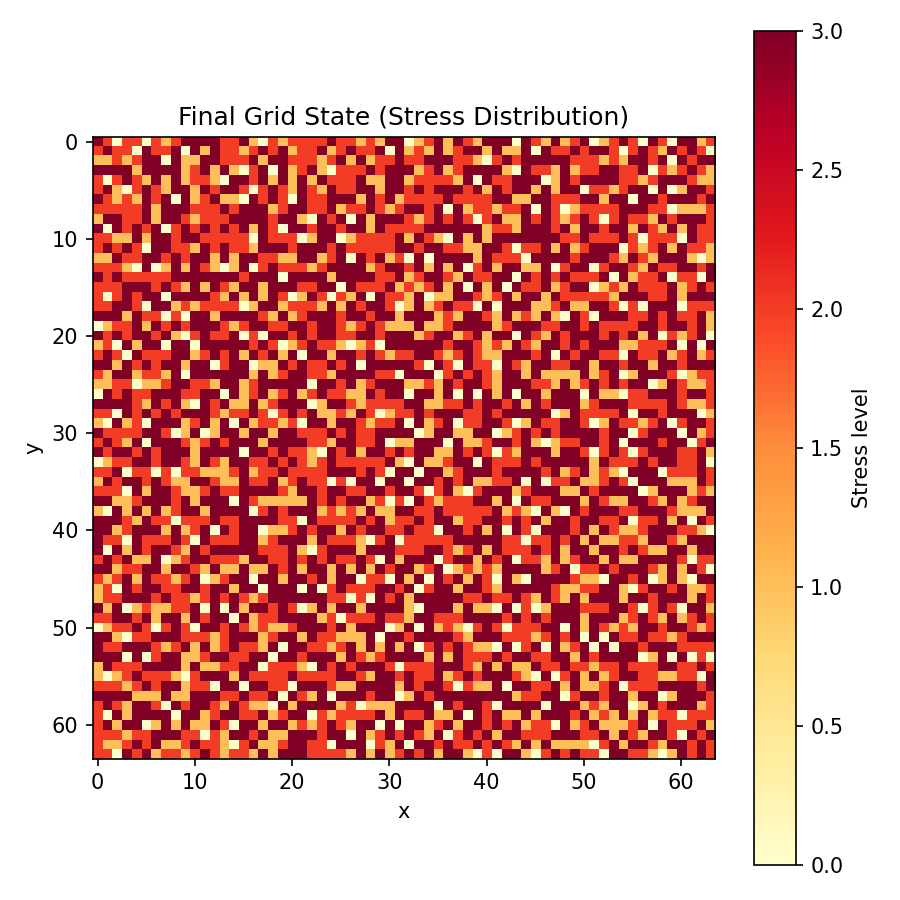
\includegraphics[width=0.5\textwidth]{grid_snapshot.png}
    \caption{Snapshot of the stress field in the self-organized critical state.}
    \label{fig:grid}
\end{figure}

\section{Discussion: Self-Organized Critical State}

The simulation confirms that the BTW sandpile model, applied to earthquake
fault dynamics, exhibits self-organized criticality:

\begin{enumerate}
    \item \textbf{No parameter tuning}: The system reaches the critical state
          solely through the interplay of slow driving (random stress
          accumulation) and fast relaxation (avalanches). No temperature,
          coupling constant, or other control parameter needs to be adjusted.
    \item \textbf{Power-law distributions}: Both avalanche sizes and durations
          follow power laws over several decades, indicating the absence of
          a characteristic scale---the hallmark of criticality.
    \item \textbf{Separation of time scales}: The driving time scale (one grain
          per step) is much slower than the relaxation time scale (avalanches
          complete before the next grain is added), satisfying a key condition
          for SOC.
    \item \textbf{Universality}: The measured exponents ($\tau \approx 1.1$,
          $\alpha \approx 1.25$) are consistent with the 2D BTW universality
          class, suggesting that the macroscopic behavior is robust to
          microscopic details.
\end{enumerate}

The analogy to real earthquakes is compelling: the Gutenberg-Richter law's
power-law magnitude distribution, the fractal spatial structure of fault
networks, and the complex aftershock sequences all emerge naturally from
SOC dynamics. However, real fault systems include complications such as
heterogeneous material properties, viscoelastic relaxation, and
rate-and-state friction that are not captured by this simple model.

\section{Conclusion}

We have demonstrated that the BTW sandpile model successfully captures
the essential features of self-organized criticality in earthquake fault
networks. The power-law distributions of avalanche sizes and durations,
the scaling relations between size and spatial connectivity, and the
spontaneous organization to a critical state all emerge from minimal
local rules without external parameter tuning. This supports the view
that SOC provides a useful framework for understanding the statistical
properties of earthquakes and other complex geophysical phenomena.

\section*{Acknowledgments}

This project was completed with the assistance of Claude (Anthropic),
an AI assistant, which helped with code development, data analysis,
and manuscript preparation.

\section*{List of Prompts Used}

The following prompts were used with Claude (Anthropic) during the
development of this project:
\begin{enumerate}
    \item ``I have to do a project in C++ for my course. [Full assignment
          description]. Please create the simulation code, analysis scripts,
          and LaTeX report for a complexity science project applying
          self-organized criticality to earthquake fault dynamics using the
          BTW sandpile model.''
          \item "Explain why earthquake fault networks satisfy the criteria for complex systems and how noise, avalanches, and connectivity manifest in real seismological settings."
          \item "Implement the BTW sandpile model in C++ with open boundary conditions on a 64×64 lattice. Track avalanche size, duration, unique sites toppled, and maximum spatial radius for each event."
\end{enumerate}

\bibliographystyle{plainnat}
\begin{thebibliography}{9}

\bibitem[Bak et~al.(1987)]{bak1987}
P.~Bak, C.~Tang, and K.~Wiesenfeld.
\newblock Self-organized criticality: An explanation of the 1/f noise.
\newblock \textit{Physical Review Letters}, 59(4):381--384, 1987.

\bibitem[Bak(2002)]{bak2002}
P.~Bak.
\newblock \textit{How Nature Works: The Science of Self-Organized Criticality}.
\newblock Copernicus Books, 2002.

\bibitem[Gutenberg and Richter(1944)]{gutenberg1944}
B.~Gutenberg and C.~F. Richter.
\newblock Frequency of earthquakes in California.
\newblock \textit{Bulletin of the Seismological Society of America},
  34(4):185--188, 1944.

\bibitem[L{\"u}beck(2004)]{lubeck2004}
S.~L{\"u}beck.
\newblock Universal scaling behavior of non-equilibrium phase transitions.
\newblock \textit{International Journal of Modern Physics B},
  18(31--32):3977--4118, 2004.

\bibitem[Olami et~al.(1992)]{olami1992}
Z.~Olami, H.~J.~S. Feder, and K.~Christensen.
\newblock Self-organized criticality in a continuous, nonconservative cellular
  automaton modeling earthquakes.
\newblock \textit{Physical Review Letters}, 68(8):1244--1247, 1992.

\end{thebibliography}

\end{document}
